\documentclass[uplatex,a4j,11pt,dvipdfmx]{jsarticle}
\usepackage{listings,jvlisting}
\bibliographystyle{junsrt}

\usepackage{url}

\usepackage{graphicx}
\usepackage{gnuplot-lua-tikz}
\usepackage{pgfplots}
\usepackage{tikz}
\usepackage{amsmath,amsfonts,amssymb}
\usepackage{bm}
\usepackage{siunitx}
\usepackage{braket}

\makeatletter
\def\fgcaption{\def\@captype{figure}\caption}
\makeatother
\newcommand{\setsections}[3]{
\setcounter{section}{#1}
\setcounter{subsection}{#2}
\setcounter{subsubsection}{#3}
}
\newcommand{\mfig}[3][width=15cm]{
\begin{center}
\includegraphics[#1]{#2}
\fgcaption{#3 \label{fig:#2}}
\end{center}
}
\newcommand{\gnu}[2]{
\begin{figure}[hptb]
\begin{center}
\input{#2}
\caption{#1}
\label{fig:#2}
\end{center}
\end{figure}
}
\newcommand{\up}{\uparrow}
\newcommand{\dn}{\downarrow}

\begin{document}
\title{統計物理学 No.2}
\author{82311971 佐々木良輔}
\date{}
\maketitle
\subsection*{(a)}
2スピン系のXXZ相互作用ハミルトニアンは
\begin{align}
  \begin{split}
    H&=J(S_1^xS_2^x+S_1^yS_2^y+\Delta S_1^zS_2^z)-h(S_1^z+S_2^z)\\
    &=\frac{J}{2}(S_1^+S_2^-+S_2^+S_1^-)+J\Delta S_1^zS_2^z-h(S_1^z+S_2^z)
  \end{split}
\end{align}
である.このとき
\begin{align}
  \begin{split}
    H\Ket{\up\up}&=\frac{J}{2}\left(0\otimes S_2^-\Ket{\up}+0\otimes S_1^-\Ket{\up}\right)+J\Delta S_1^z\Ket{\up}\otimes S_2^z\Ket{\up}-h\left(S_1^z\Ket{\up}\otimes\Ket{\up}+\Ket{\up}\otimes S_2^z\Ket{\up}\right)\\
    &=0+J\Delta\frac{1}{2}\Ket{\up}\otimes\frac{1}{2}\Ket{\up}-h\left(\frac{1}{2}\Ket{\up}\otimes\Ket{\up}+\Ket{\up}\otimes\frac{1}{2}\Ket{\up}\right)\\
    &=\left(\frac{J\Delta}{4}-h\right)\Ket{\up\up}
  \end{split}
\end{align}
\begin{align}
  \begin{split}
    H\Ket{\dn\dn}&=\frac{J}{2}\left(S_1^+\Ket{\dn}\otimes0+S_2^+\Ket{\dn}\otimes0\right)+J\Delta S_1^z\Ket{\dn}\otimes S_2^z\Ket{\dn}-h\left(S_1^z\Ket{\dn}\otimes\Ket{\dn}+\Ket{\dn}\otimes S_2^z\Ket{\dn}\right)\\
    &=0+J\Delta\left(-\frac{1}{2}\Ket{\dn}\right)\otimes\left(-\frac{1}{2}\Ket{\dn}\right)
    -h\left(\left(-\frac{1}{2}\Ket{\dn}\right)\otimes\Ket{\dn}+\Ket{\dn}\otimes\left(-\frac{1}{2}\Ket{\dn}\right)\right)\\
    &=\left(\frac{J\Delta}{4}+h\right)\Ket{\dn\dn}
  \end{split}
\end{align}
\begin{align}
  \begin{split}
    H\Ket{\up\dn}&=\frac{J}{2}\left(0\otimes0+S_2^+\Ket{\dn}\otimes S_1^-\Ket{\up}\right)+J\Delta S_1^z\Ket{\up}\otimes S_2^z\Ket{\dn}-h\left(S_1^z\Ket{\up}\otimes\Ket{\dn}+\Ket{\up}\otimes S_2^z\Ket{\dn}\right)\\
    &=\frac{J}{2}\Ket{\dn}\otimes\Ket{\up}+J\Delta\frac{1}{2}\Ket{\up}\otimes\left(-\frac{1}{2}\Ket{\dn}\right)-h\left(\frac{1}{2}\Ket{\up}\otimes\Ket{\dn}+\Ket{\up}\otimes\left(-\frac{1}{2}\Ket{\dn}\right)\right)\\
    &=\frac{J}{2}\Ket{\dn\up}-\frac{J\Delta}{4}\Ket{\up\dn}
  \end{split}
\end{align}
\begin{align}
  \begin{split}
    H\Ket{\dn\up}&=\frac{J}{2}\left(S_1^+\Ket{\dn}\otimes S_2^-\Ket{\up}+0\otimes0\right)+J\Delta S_1^z\Ket{\dn}\otimes S_2^z\Ket{\up}-h\left(S_1^z\Ket{\dn}\otimes\Ket{\up}+\Ket{\dn}\otimes S_2^z\Ket{\up}\right)\\
    &=\frac{J}{2}\Ket{\up}\otimes\Ket{\dn}+J\Delta\left(-\frac{1}{2}\Ket{\dn}\right)\otimes\frac{1}{2}\Ket{\up}-h\left(\left(-\frac{1}{2}\Ket{\dn}\right)\otimes\Ket{\up}+\Ket{\dn}\otimes\frac{1}{2}\Ket{\up}\right)\\
    &=\frac{J}{2}\Ket{\up\dn}-\frac{J\Delta}{4}\Ket{\dn\up}
  \end{split}
\end{align}
である.ここで
\begin{align}
  \begin{split}
    \Ket{t_{+1}}=\Ket{\up\up},\ 
    \Ket{t_{-1}}=\Ket{\dn\dn},\ 
    \Ket{t_0}=\frac{1}{\sqrt{2}}\left(\Ket{\up\dn}+\Ket{\dn\up}\right),\ 
    \Ket{s}=\frac{1}{\sqrt{2}}\left(\Ket{\up\dn}-\Ket{\dn\up}\right)
  \end{split}
\end{align}
は固有状態であり,それぞれの固有値は
\begin{align}
  H\Ket{t_{+1}}=\left(\frac{J\Delta}{4}-h\right)\Ket{t_{+1}}
\end{align}
\begin{align}
  H\Ket{t_{-1}}=\left(\frac{J\Delta}{4}+h\right)\Ket{t_{-1}}
\end{align}
\begin{align}
  \begin{split}
    H\Ket{t_0}&=\frac{1}{\sqrt{2}}\left(\frac{J}{2}\left(\Ket{\up\dn}-\Ket{\dn\up}\right)-\frac{J\Delta}{4}\left(\Ket{\up\dn}+\Ket{\dn\up}\right)\right)\\
    &=\left(\frac{J}{2}-\frac{J\Delta}{4}\right)\Ket{t_0}
  \end{split}
\end{align}
\begin{align}
  \begin{split}
    H\Ket{s}&=\frac{1}{\sqrt{2}}\left(-\frac{J}{2}\left(\Ket{\up\dn}-\Ket{\dn\up}\right)-\frac{J\Delta}{4}\left(\Ket{\up\dn}+\Ket{\dn\up}\right)\right)\\
    &=-\left(\frac{J}{2}+\frac{J\Delta}{4}\right)\Ket{s}
  \end{split}
\end{align}
となる.
\subsection*{(b)(i)}
$\Ket{t_{\pm1}}$のエネルギーは$h=0$において$J\Delta/4$である.
$\Delta\geq1$のとき$h\geq0$において$E_{t_{+1}}$は$E_{t_0}$, $E_s$とそれぞれ一回ずつ交点をもち,その値は
\begin{align}
  \begin{array}{cc}
    &\cfrac{J\Delta}{4}-h=\cfrac{J}{2}-\cfrac{J\Delta}{4}\\
    \iff&h=\cfrac{J}{2}(\Delta-1)
  \end{array}
\end{align}
\begin{align}
  \begin{array}{cc}
    &\cfrac{J\Delta}{4}-h=-\cfrac{J}{2}-\cfrac{J\Delta}{4}\\
    \iff&h=\cfrac{J}{2}(\Delta+1)
  \end{array}
\end{align}
である.したがってエネルギースペクトルは図1のようになる.図1から$h\leq J/2(\Delta+1)$での基底状態は$\Ket{s}$,
$h>J/2(\Delta+1)$での基底状態は$\Ket{t_{+1}}$である.それぞれの状態での磁化の期待値は
\begin{align}
  \begin{split}
    \Braket{s|S_1^z+S_2^z|s}&=\Bra{s}(S_1^z+S_2^z)\frac{1}{\sqrt{2}}\left(\Ket{\up\dn}-\Ket{\dn\up}\right)\\
    &=\Bra{s}\frac{1}{\sqrt{2}}\left(S_1^z\Ket{\up\dn}-S_1^z\Ket{\dn\up}+S_2^z\Ket{\up\dn}-S_2^z\Ket{\dn\up}\right)\\
    &=\Bra{s}\frac{1}{\sqrt{2}}\left(\frac{1}{2}\Ket{\up\dn}+\frac{1}{2}\Ket{\dn\up}-\frac{1}{2}\Ket{\up\dn}-\frac{1}{2}\Ket{\dn\up}\right)\\
    &=0
  \end{split}
\end{align}
\begin{align}
  \begin{split}
    \Braket{t_{+1}|S_1^z+S_2^z|t_{+1}}&=\Bra{\up\up}(S_1^z+S_2^z)\Ket{\up\up}\\
    &=\Bra{\up\up}\left(\frac{1}{2}+\frac{1}{2}\right)\Ket{\up\up}=1
  \end{split}
\end{align}
したがって磁化の期待値は図2のように振る舞う.
\begin{center}
  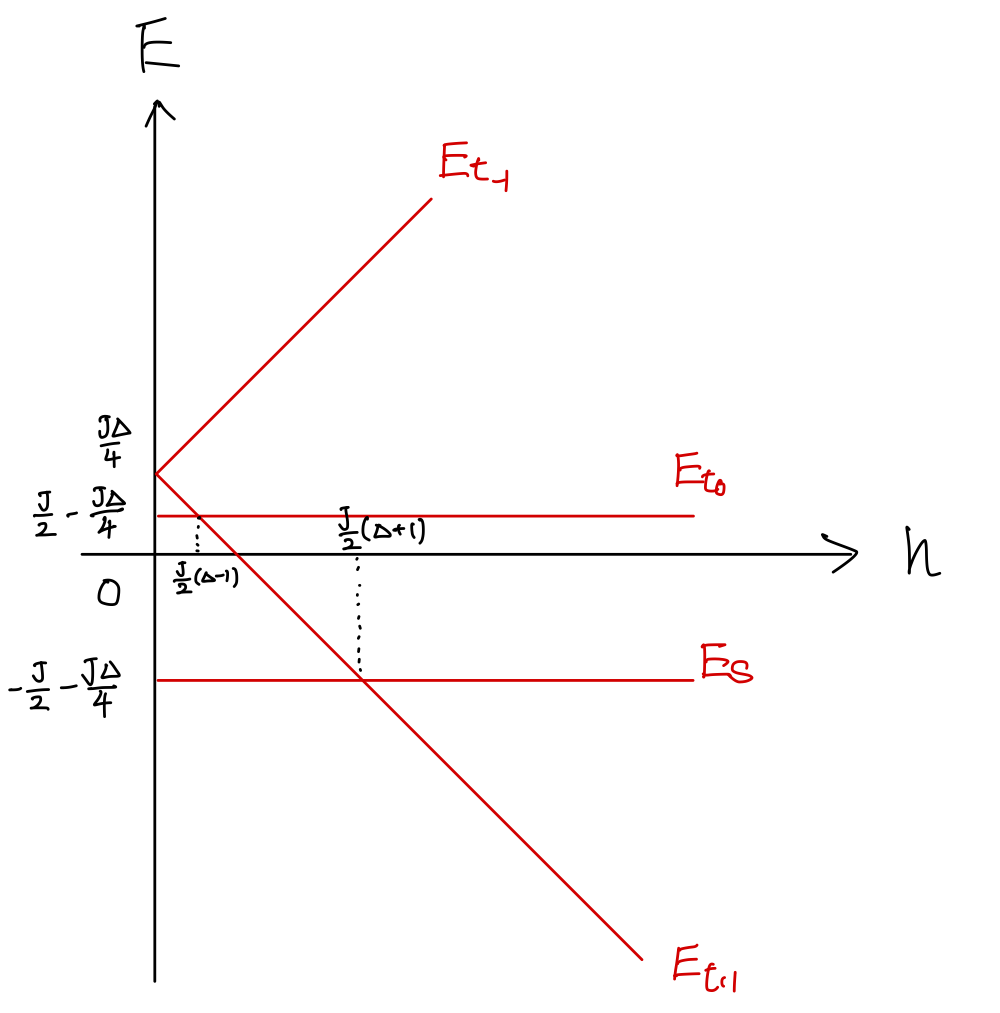
\includegraphics[width=8cm]{espec_dgeq0.png}
  \fgcaption{$\Delta\geq1$の場合のエネルギースペクトル}
\end{center}
\begin{center}
  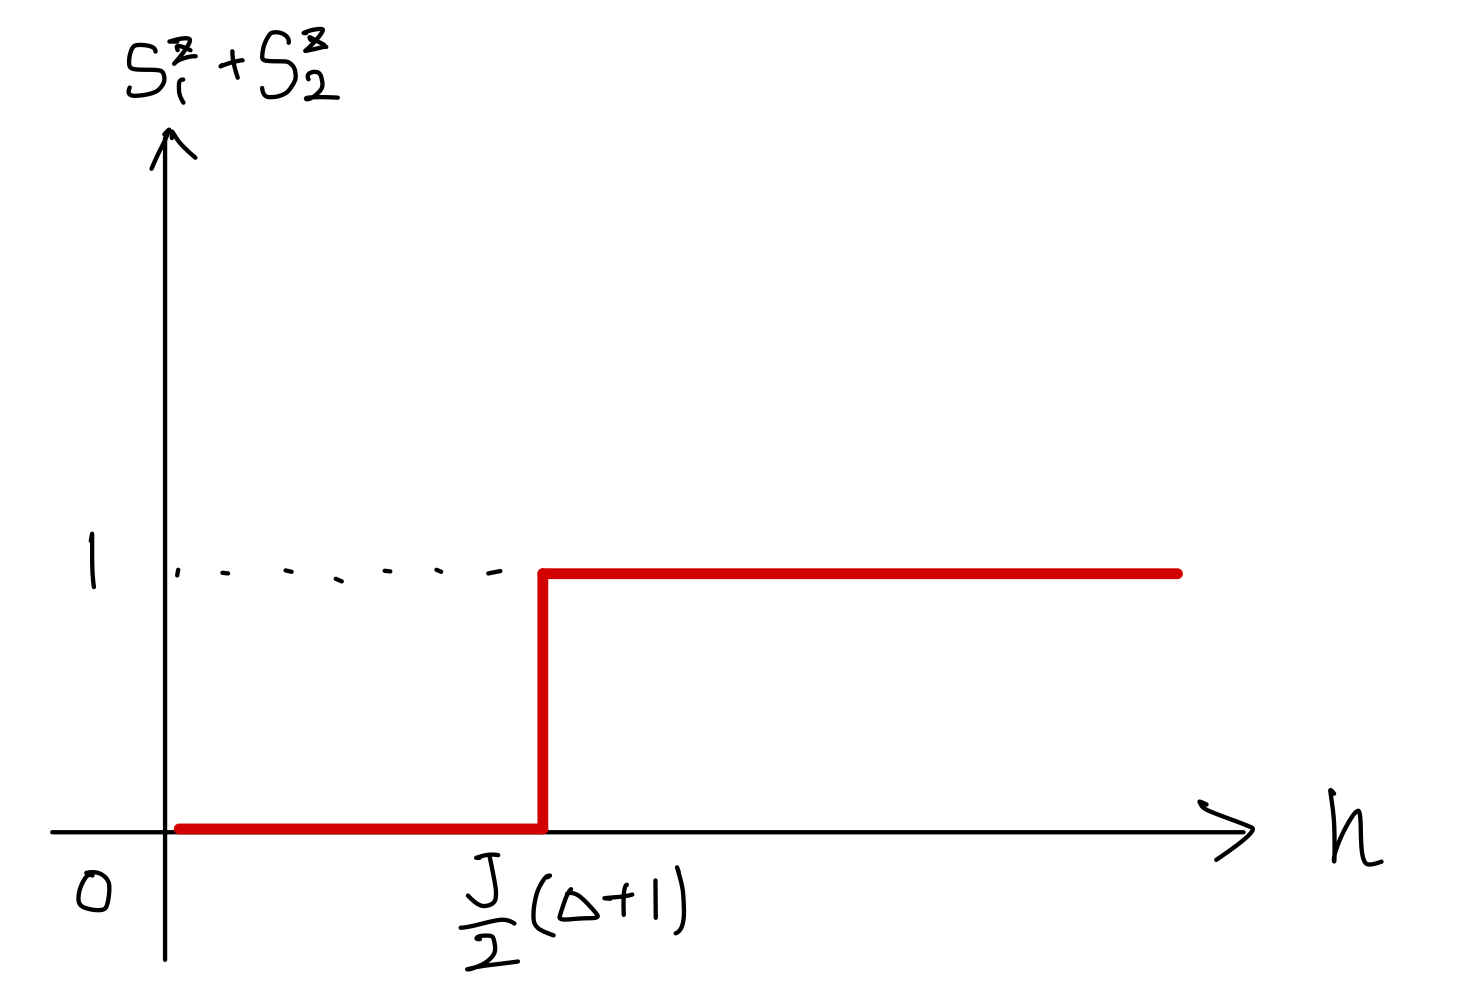
\includegraphics[width=8cm]{mspec_dgeq0.png}
  \fgcaption{$\Delta\geq1$の場合の磁化の期待値}
\end{center}
\subsection*{(b)(ii)}
\bibliography{ref.bib}
\end{document}